\subsection*{pulley system 3}

\begin{center}
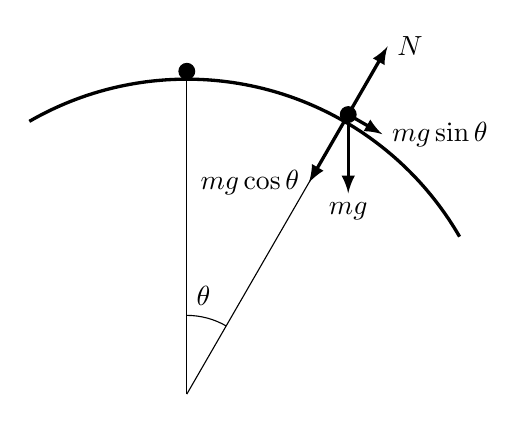
\begin{tikzpicture}[scale=1]

\draw [very thick] (0,4) arc [start angle=90, end angle= 30, radius = 4] ;
\draw [very thick] (0,4) arc [start angle=90, end angle= 120, radius = 4] ;
\draw (0,0) -- (0,4) ;
\draw [fill] (0,4.1) circle [radius=0.1] ; 
\draw [fill] (60:4.1) circle [radius=0.1] ;
\draw (0,0) -- (60:4) ;
\draw (0,1) arc [start angle =90, end angle=60,radius=1] ;
\draw (0,1) node [anchor=south west] {$\theta$} ;
\draw [very thick,-{latex}] (60:4.1) -- ++(0,-1) ;
\draw (60:4.1) ++(0,-1) node [anchor=north] {$mg$} ;
\draw [very thick,-{latex}] (60:4.1) -- ++(-120:1) ;
\draw (60:4.1) ++(-120:1) node [anchor=east] {$mg\cos\theta$} ;
\draw [very thick,-{latex}] (60:4.1) -- ++(60:1) ;
\draw (60:4.1) ++(-30:0.5) node [anchor=west] {$mg\sin\theta$} ;
\draw [very thick,-{latex}] (60:4.1) -- ++(-30:0.5) ;
\draw (60:4.1) ++(60:1) node [anchor=west] {$N$} ;

\end{tikzpicture}
\end{center}
